\chapter{Parameters optimization}\label{optimization}
Code FAINA allows not only to evaluate radiation from the source, but also to fit model data to observations and obtain parameters of the source. There are various types optimization methods and models of loss functions, implemented in the code.

\section{Evaluators of the loss function}

The first thing one should determine to start optimization process is a loss function. In FAINA code abstract class LossEvalator and derived classes are used for it. All implemented classes use quadratic loss functions, taking into account observational errors:
$L = \sum \frac{(F_i - F_{obs,i})^2}{\sigma_i^2}$, where $F_i$ - is some modeled function of radiation (e.g. energy spectral density) evaluated at point corresponding to some observation, $F_{obs,i}$ - observed value of this function, $\sigma_i$ - it's uncertancy. There are following classes of loss function evaluator implemented in the cod: SpectrumLossEvaluator - for fitting energy flux spectral density in given time moment, TimeDependentSpectrumLossEvaluator - for fitting energy flux spectal density in different time moments and RadialProfileLossEvaluator - for fitting luminocity of the prolonged source in different points depending on radius in tangent plane. Public methods of this classes are listed in Table \ref{LossEvaluators}.

\begin{small}
	\topcaption{Public methods of loss function evaluators}
	\label{LossEvaluators}
	\begin{xtabular}{|p{0.5\textwidth}|p{0.5\textwidth}|}
		\hline
		\textbf{LossEvaluator} & abstract class for evaluator of loss function\\
		\hline
		virtual double evaluate(const double* vector, const double* maxParameters, RadiationEvaluator* evaluator) & virtual method, returns value of loss function with given parameters. Also takes vector of normalization units for parameters and radiation evaluator\\
		\hline
		\textbf{SpectrumLossEvaluator} & class for fitting energy flux energy density. Loss function is $L = \sum \frac{(F(E_i) - F_{obs,i})^2}{\sigma_i^2}$, where $F(E_i)$ - modeled energy flux energy density evaluated at energy $E_i$, $F_{obs,i}$ - corresponding observed value, $\sigma_i$ - it's uncertancy.\\
		\hline
		SpectrumLossEvaluator(double* energy, double* observedFlux, double* observedError, int Ne, RadiationSource* radiatiornSource) & constructor, creates loss evaluator, with given values of energies of observational points, observed fluxes and it's uncertancies, number of points and radiation source\\
		\hline
		\textbf{TimeDependentSpectrumLossEvaluator} & class fitting energy flux energy density at different time moments. Loss function is $L = \sum \frac{(F(E_{ij}, t_j) - F_{obs,i,j})^2}{\sigma_{ij}^2}$, where $F(E_{ij},t_j)$ - modeled energy flux energy density evaluated at energy $E_{ij}$ at time moment $t_j$, $F_{obs,i,j}$ - corresponding observed value, $\sigma_{ij}$ - it's uncertancies. NOTE that number of energy grid point may be different at different time moments\\
		\hline
		TimeDependentSpectrumLossEvaluator(double** energy, double** observedFlux, double** observedError, int* Ne, double* times, int Ntimes, RadiationTimeDependentSource* radiationSource) & constructor, creates loss evaluator with given values of energies of observational points, observed fluxes and it's uncertancies, numbers of energy grid points, time moments, number of time grid points and radiation source\\
		\hline
		\textbf{RadialProfileLossEvaluator} & class for fitting luminocity of different points of the source, depending of radius in tangent plane. Loss function is $L = \sum \frac{(F(R_i) - F_{obs,i})^2}{\sigma_i^2}$, where $F(R_i)$ - energy flux surface density, at given radius $R_i$, $F_{obs,i}$ - corresponding observed value, $\sigma_i$ - it's uncertancy\\
		\hline
		RadialProfileLossEvaluator(double energy, double* observedFlux, double* observedError, double* rhoPoints, int Nrho, RadiationSource* radiaionSource) & constructor, creates loss evaluator, wuth given value of energy to evaluate flux density, observed value of luminocity surface density, observed value and it's uncertancies, radius grid points, number of grid points and radiation source\\
		\hline
	\end{xtabular}
\end{small}

\section{Optimizers of loss function}

For fitting modeled radiation from the source to observational data, abstract class RadiationOptimizer is implemented. It has virtual function optimize(double* vector, bool* optPar) which performs minimization of loss function. This function takes on input array of parameters of the source vector, and boolean array optPar showing for each parameter to optimize it or consider it fixed. Array of parameters must be consistent with function of used radiation source resetParameters, which was described in section \ref{sourcesSection}, because this function will be used during optimization and take the same array of parameters as input.

There are three implemented classes, inherited from RadiationOptimizer: GridEnumRadiationOptimizer, which finds minimum of loss function on the fixed logarithmic grid in the parameters space, GradientDescentRadiationOptimizer, which uses gradient descent method and CombinedRadiationOptimizer, which sequentially applies this method, using result of seqrch on the grid as starting point for gradient descent. Hierarchy scheme of optimizers classes is shown in Figure \ref{radiationOptimizer}, and public methods are listed in Table \ref{RadiationOptimizerMethods}. Implemented optimization methods can be applied to any types of sources, electro-magnetic radiation and loss function evaluators which were described above.
\begin{figure}
	\centering
	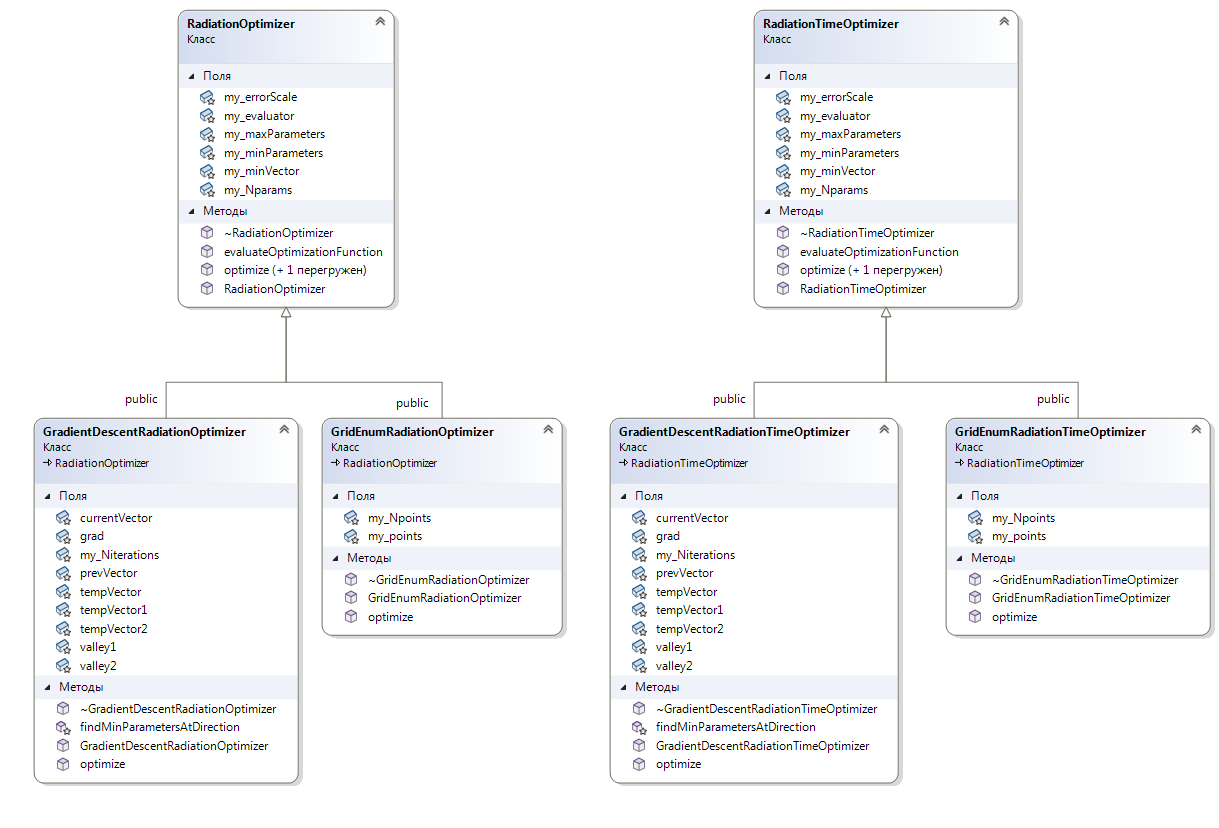
\includegraphics[width=11.5 cm]{./fig/radiationOptimizer.png} 
	\caption{class hierarchy of radiation optimizers}
	\label{radiationOptimizer}
\end{figure}

\begin{small}
	\topcaption{Public methods of radiation optimizer classes}
	\label{RadiationOptimizerMethods}
	\begin{xtabular}{|p{0.41\textwidth}|p{0.59\textwidth}|}
		\hline
		\textbf{RadiationOptimizer} & abstract class for fitting modeled radiation to observations and optimization of source parameters \\
		\hline
		double evaluateOptimizationFunction( const double* vector) & returns value of loss function with given parameters\\
		\hline
		void optimize( double* vector, bool* optPar) & performs optimization, takes array of peremeters, where final values would be writen, and array of boolean values showing to optimize corresponding parameter or consider it fixed \\
		\hline
		void outputProfileDiagrams( const double* vector, int Npoints) & evaluates and writes into files 2d profiles of loss function in parameters space which contain starting point, defined by array vector, for all possible pairs of parameters\\
		\hline
		void outputOptimizedProfileDiagram( const double* vector, bool* optPar, int Npoints, int Nparam1, int Nparam2) & evaluates and writes into file 2d profile of loss function in plane in the parameter space, defined by parameter numbers Nparam1 and Nparam2, containing starting point in it, with given nuber of grid points for this parameters, while other parameters are optimized, if it is allowed by boolean array optPar\\
		\hline
		\textbf{GridEnumRadiationOptimizer} & class for optimization by search of minimum value on the fixed logarithmic grid in parameters space\\
		\hline
		GridEnumRadiationOptimizer( RadiationEvaluator* evaluator, const double* minParameters, const double* maxParameters, int Nparams, const int* Npoints, LossEvaluator* lossEvaluator) & constructor, creates optimizer with given radiation evaluator, domain of parameters defined by minimum and maximum values, number of parameters, numbers of grid points for each parameters and loss function evaluator\\
		\hline
		\textbf{GradientDescentRadiationOptimizer} & class for optimization with gradient descent method\\
		\hline
		GradientDescentRadiationOptimizer( RadiationEvaluator* evaluator, const double* minParameters, const double* maxParameters, int Nparams, int Niterations, LossEvaluator* lossEvaluator) & constructor, creates optimizer with given radiation evaluator, domain of parameters defined by minimum and maximum values, number of parameters, number of iterations of gradient descent and loss function evaluator\\
		\hline
		\textbf{CombinedRadiationOptimizer} & class for optimization with sequentially use of search of minimum on the fixed grid and gradient descent method\\
		\hline
		CombinedRadiationOptimizer( RadiationEvaluator* evaluator, const double* minParameters, const double* maxParameters, int Nparams, int Niterations, const int* Npoints, LossEvaluator* lossEvaluator) & constructor, creates optimizer with given radiation evaluator, domain of parameters defined by minimum and maximum values, number of parameters, number of iterations for gradient descent, number of pointes through each axis for gread search and loss function evaluator\\
		\hline
	\end{xtabular}
\end{small}

Example of optimizing the source parameters with fitting radiation to observationsl data is shown in the function fitCSS161010withPowerLawDistribition in file examples.cpp. Following the work \cite{Coppejans2020} let evaluate synchrotron radiation from the source taking into account synchrotron self-absorption, considering power-law distribution of enitting electrons with index 3.6. But we will not fix such parameters as efractios of energy in magnetic field and accelerated electrons, instead we consider magnetic field and electrons concentration independent parameters, wich optimal values will be found with fitting.

Let optimize parameters of the source of Fast Blue Optical Transient CSS161010 at 98 day after explosion. We initialize source parameters using values from \cite{Coppejans2020}, they will be used as starting point of optimization.

\begin{lstlisting}[language=c++]
    double electronConcentration = 25;
    double B = 0.6;
    double R = 1.4E17;
    double fraction = 0.5;
    const double distance = 150 * 1E6 * parsec;
\end{lstlisting}

Then we create power-law distribution of emitting electrons with index 3.6, radiation source as homogenous disk and synchrotron radiation evaluator

\begin{lstlisting}[language=c++]
    double Emin = me_c2;
    double Emax = 10000 * me_c2;
    double index = 3.6;
	
    SynchrotronEvaluator* synchrotronEvaluator = new
        SynchrotronEvaluator(200, Emin, Emax);

    MassiveParticlePowerLawDistribution* electrons = 
        new MassiveParticlePowerLawDistribution(
        massElectron, index, Emin, electronConcentration);

    SimpleFlatSource* source = new
        SimpleFlatSource(electrons, B, pi/2, R, fraction * R, distance);
\end{lstlisting}

Now we define vector of parameters to be optimized - radius of the source, magnetic field, electron's number density and width fraction of the source. This parameters correspond to the resetParameters function of class SimpleFlatSource. Also one should define search domain with minimum and maximum value of each parameter. Maximum values are also used as normaliztion units.

\begin{lstlisting}[language=c++]
    const int Nparams = 4;
    double minParameters[Nparams] = { 1E17, 0.01, 0.5, 0.1 };
    double maxParameters[Nparams] = { 2E17, 10, 200, 1.0 };
    double vector[Nparams] = { R, B, electronConcentration, fraction};
    for (int i = 0; i < Nparams; ++i) {
	    vector[i] = vector[i] / maxParameters[i];
    }
\end{lstlisting}

Also we create arrays of observational data, which should be fitted. Note, the frequency should be transformed to energy, and flux spectral density to the flux energy density (to the units $\text{cm}^{-2}\text{s}^{-1}$). 
\begin{lstlisting}[language=c++]
    const int Nenergy1 = 4;
    double energy1[Nenergy1] = { 1.5E9*hplank, 3.0E9 * hplank, 
    	6.1E9 * hplank, 9.8E9 * hplank };
    double observedFlux[Nenergy1] = { 1.5/(hplank*1E26), 
    	4.3/(hplank*1E26), 6.1/(hplank*1E26), 4.2 /(hplank*1E26)};
    double observedError[Nenergy1] = { 0.1 / (hplank * 1E26), 
    	0.2/(hplank*1E26), 0.3/(hplank*1E26), 0.2/(hplank*1E26)};
\end{lstlisting}
Then we create evaluator of loss function and combined optimizer. We define number of grid points to search and number of gradient descent iterations. Also we create array of boolean showing that all parameters should be optimized.
\begin{lstlisting}[language=c++]
    bool optPar[Nparams] = { true, true, true, true };
    int Niterations = 20;
    int Npoints[Nparams] = { 10,10,10,10 };
    
    LossEvaluator* lossEvaluator = new SpectrumLossEvaluator(energy1, observedFlux, observedError, Nenergy1, source);
    RadiationOptimizer* optimizer = new CombinedRadiationOptimizer(
        synchrotronEvaluator,minParameters,maxParameters,Nparams, Niterations,Npoints, lossEvaluator);
\end{lstlisting}
Let call function optimize and reset source parameters to obtained optimal values.
\begin{lstlisting}[language=c++]
    optimizer->optimize(vector, optPar, energy1, observedFlux, 
        observedError, Nenergy1, source);
    source->resetParameters(vector, maxParameters);
\end{lstlisting}
Jbtained optimal values of source parameters are: disk radius $R = 1.8\times10^17 \text{ см}$, magnetic field $B = 1.6 \text{ Гс}$, electron's number density $n = 2.3 \text{ см}^{-3}$, width fraction $fraction = 0.54 $. 
Modeled spectrum of synchrotron radiation of source with this parameters and observational data are shown in Figure \ref{synchrotron1}.
\begin{figure}[h]
	\centering
	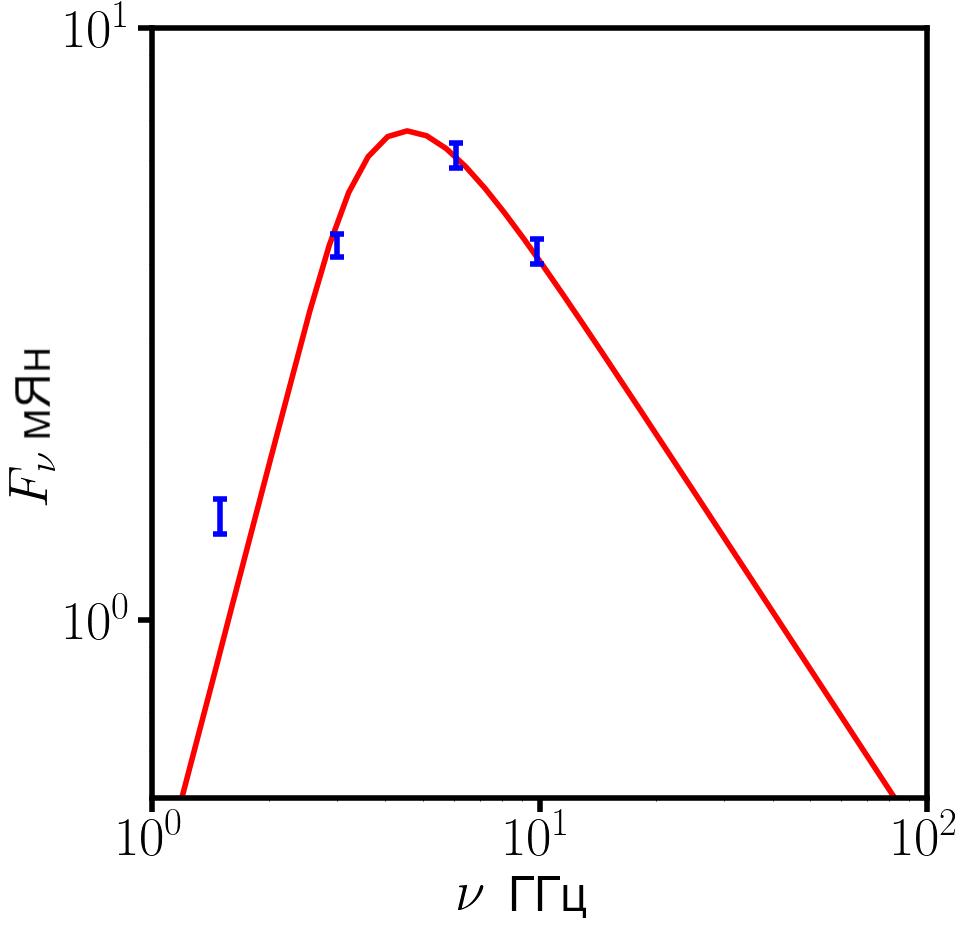
\includegraphics[width=12.5 cm]{./fig/synchrotron1.png} 
	\caption{Modeled spectrum of synchrotron radiation and observational data for CSS161010 at 98 day after explosion}
	\label{synchrotron1}
\end{figure}


%Пример фитирования параметров источника по наблюдательным данным приведен в функции fitTimeDependentCSS161010() в файле examples.cpp. Подберем параметры Быстрого Оптического Голубого Транзиента CSS161010 на основе наблюдений радиоизлучения, проведенных на 98, 162, 357 день после вспышки.  Расчет синхротронного излучения учитывает самопоглощение и раширение источника. Источник будем считать шаровым слоем с однородной плотностью и однороным магнитным полем, направленным перпендикулярно лучу зрения. Функцию распределения излучающих электронов возьмем на основе Particle-in-Cell расчетов для ударной волны со скоростью 0.3c,как сделано в работе \cite{BykovUniverse}. Учтена зависимость функции распределения от угла между магнитным полем и направлением распространения ударной волны.

%Подберем параметры Быстрого Оптического Голубого Транзиента CSS161010 на основе наблюдений радиоизлучения, проведенных на 98, 162, 357 день после вспышки.  Зададим сначала массивы наблюдательных точек, переведя при этом из единиц герцы и милиянские в эрги и $\text{см}^{-2} \text{c}^{-1}$
%\begin{lstlisting}[language=c++]
%const double cssx1[4] = 
%{1.5*hplank*1E9, 3.0*hplank*1E9, 6.1*hplank*1E9, %9.87*hplank*1E9};
%const double cssy1[4] =  {1.5/(hplank*1E26), 
%4.3/(hplank*1E26), 6.1/(hplank*1E26), 4.2/(hplank*1E26)};
%const double cssError1[4] = {0.1/(hplank*1E26), 
%0.2/(hplank*1E26), 0.3/(hplank*1E26), 0.2/(hplank*1E26)};
	
%const double cssx2[4] = 
%{2.94*hplank*1E9, 6.1*hplank*1E9, 9.74*hplank*1E9, %22.0*hplank*1E9};
%const double cssy2[4] = {2.9/(hplank*1E26), 
%2.3/(hplank*1E26), 1.74/(hplank*1E26), %0.56/(hplank*1E26)};
%const double cssError2[4] = {0.2/(hplank*1E26), 
%0.1/(hplank*1E26), 0.09/(hplank*1E26), %0.03/(hplank*1E26)};
	
%const double cssx3[6] = {0.33*hplank*1E9, %0.61*hplank*1E9, 
%1.5*hplank*1E9, 3.0*hplank*1E9, 6.05*hplank*1E9, %10.0*hplank*1E9};
%const double cssy3[6] = {0.375/(hplank*1E26), %0.79/(hplank*1E26), 
%0.27/(hplank*1E26),0.17/(hplank*1E26),0.07/(hplank*1E26),0.32/(hplank*1E27)};
%const double cssError3[6] = {0.375/(hplank*1E26), 0.09/(hplank*1E26),
%0.07/(hplank*1E26),0.03/(hplank*1E26),0.01/(hplank*1E26),0.8/(hplank * 1E28)};
%\end{lstlisting}

%Определим моменты времени инаблюдений и соответствующие им количества точек

%\begin{lstlisting}[language=c++]
%const int Ntimes = 3;
%double times[Ntimes] = { 99 * 24 * 3600, 162 * 24 * 3600, 357 * 24 * 3600 };
%int Nenergy[Ntimes];
%Nenergy[0] = 4;
%Nenergy[1] = 4;
%Nenergy[2] = 6;
%\end{lstlisting}
%Создадим и инициализируем необходимые массивы с наблюдательными данными
%\begin{lstlisting}[language=c++]
%double** energy = new double* [Ntimes];
%double** F = new double* [Ntimes];
%double** Error = new double* [Ntimes];
%for (int m = 0; m < Ntimes; ++m) {
%	energy[m] = new double[Nenergy[m]];
%	F[m] = new double[Nenergy[m]];
%	Error[m] = new double[Nenergy[m]];
%}

%for (int i = 0; i < Nenergy[0]; ++i) {
%	energy[0][i] = cssx1[i];
%	F[0][i] = cssy1[i];
%	Error[0][i] = cssError1[i];
%}

%for (int i = 0; i < Nenergy[1]; ++i) {
%	energy[1][i] = cssx2[i];
%	F[1][i] = cssy2[i];
%	Error[1][i] = cssError2[i];
%}

%for (int i = 0; i < Nenergy[2]; ++i) {
%	energy[2][i] = cssx3[i];
%	F[2][i] = cssy3[i];
%	Error[2][i] = cssError3[i];
%}
%\end{lstlisting}

%Зададим физические параметры источника (или их начальные приближения) - расстояние, размер, концентрацию, магнитное поле, долю толщины шара, занятую излучающим веществом, скорость расширения и магнетизацию.

%\begin{lstlisting}[language=c++]
%const double distance = 150 * 1E6 * parsec;
%double rmax = 1.3E17;
%double electronConcentration = 150;
%double B = 0.6;
%double widthFraction = 0.5;
%double v = 0.3 * speed_of_light;
%double sigma = B * B / (4 * pi * massProton * 
%electronConcentration * speed_of_light2);
%\end{lstlisting}

%Укажем для оптимизаторов количество параметров, ихи минимальные и максимальные значения и соответствие вектора параметров и физических величин. Оптимизируемыми параметрами являются - размер источника, магнетизация, доля заполнения и скорость расширения в первый момент времени, а так же показатели степени расширения со временем и изменения магнитного поля и концентрации с радиусом, то есть $\alpha, \beta, \gamma$ где эти величины определены через уравнения $R(t) = R_0 + \frac{1}{\alpha-1}\cdot V(0) \cdot t_0 \cdot ({t/t_0}^{\alpha-1}-1 )$, $B(R) = B(R_0)\cdot{R_0/R}^{\beta-1}$, $n(R) = n(R_0)\cdot{R_0/R}^{\gamma - 1}$. Единица добавлена к показателям степени для удобства численных расчетов при близости величин к нулю.
%\begin{lstlisting}[language=c++]
%const int Nparams = 8;
%double minParameters[Nparams] = { 1E16, 0.0001, 0.01, 0.1, 
%0.01 * speed_of_light, 1.1, 1.0, 1.0 };
%double maxParameters[Nparams] = { 2E17, 1, 1000, 1.0, 0.6 * 
%speed_of_light, 2.0, 3.5, 3.5 };
%double vector[Nparams] = { rmax, sigma, electronConcentration, 
%widthFraction, v, 2.0, 2.0, 3.0 };
%for (int i = 0; i < Nparams; ++i) {
%    vector[i] = vector[i] / maxParameters[i];
%}
%bool optPar[Nparams] = { true, true, true, true, true, %true, true, true };
%\end{lstlisting}

%Далее создадим источник излучения. Воспользуемся моделью расширяющейся однородной сферической оболочки, с однородным магнитным полем, перпендикулярным лучу зрения и функцией распределения электронов, зависящей от угла между направлением магнитного поля и направлением расширения оболочки. Функции распределения получены с использованием Particle-in-Cell кода Smilei \cite{Derouillat} и содержатся в директории examplesData. Методика расчетов описана в статье \cite{BykovUnirse}. Количетсво распределений, посчитанных для углов от 0 до 90 градусов равно десяти. Их можно считать из соответствующих файлов, используя метод класса MassiveParticleDistributionFactory. Так же будет добавлено продолжение мтепенного хвоста, так как PIC расчеты не пользволяют получать длинные спектры из-за большой вычислительной сложности. Так же необходимо провести масштабирование распределения, так как в PIC расчетах испольовалось уменьшенное отношение масс протонов и электронов $m_p/m_e = 100$. Имея массив распределений создадим источник, учитывающий угловую зависимость, и передим его далее источнику. учитывающему зависимость от времени.

%\begin{lstlisting}[language=c++]
%const int Ndistributions = 10;

%MassiveParticleIsotropicDistribution** angleDependentDistributions = 
%MassiveParticleDistributionFactory::readTabulatedIsotropicDistributionsAddPowerLawTail
%(massElectron, "./input/Ee", "./input/Fs", ".dat", 10, 
%DistributionInputType::GAMMA_KIN_FGAMMA, electronConcentration, 200, 20 * me_c2, 3.5);
%for (int i = 0; i < Ndistributions; ++i) {
%(dynamic_cast<MassiveParticleTabulatedIsotropicDistribution*>
%(angleDependentDistributions[i]))->rescaleDistribution(sqrt(18));
%}

%AngleDependentElectronsSphericalSource* angleDependentSource = new 
%AngleDependentElectronsSphericalSource(20, 20, 4, Ndistributions, 
%angleDependentDistributions,B,1.0,0,electronConcentration,rmax,0.5*rmax,distance);

%RadiationTimeDependentSource* source = new 
%ExpandingRemnantSource(rmax, B, electronConcentration, 0.3 * speed_of_light,
%0.5, angleDependentSource, times[0]);

%\end{lstlisting}

%Теперь создадим вычислитель синхротронного излучения и два оптимизатора параметров - первый будет работать перебором параметров по сетке, а второй - градиентным спуском. Укажем количество точек по осям для перебора, количество итераций для градиентного спуска и диапазон энергий электронов, который будет рассматривать вычислитель синхротронного излучения.

%\begin{lstlisting}[language=c++]
%int Npoints[Nparams] = { 3, 3, 3, 3, 3, 3, 3, 3 };
%int Niterations = 5;

%double Emin = me_c2;
%double Emax = 10000 * me_c2;

%SynchrotronEvaluator* synchrotronEvaluator=new %SynchrotronEvaluator(200, Emin, Emax);

%RadiationTimeOptimizer* gridEnumOptimizer = 
%new GridEnumRadiationTimeOptimizer(synchrotronEvaluator, minParameters, 
%maxParameters, Nparams, Npoints);
%RadiationTimeOptimizer* gradientOptimizer = 
%new GradientDescentRadiationTimeOptimizer(synchrotronEvaluator,minParameters, 
%maxParameters, Nparams, Niterations);
%\end{lstlisting}

%Применим созданые оптимизаторы и изменим параметры источника на найденные, соответствующие минимуму.

%\begin{lstlisting}[language=c++]

%gridEnumOptimizer->optimize(vector, optPar, energy, F, Error, Nenergy, Ntimes, times, source);

%gradientOptimizer->optimize(vector, optPar, energy, F, Error, Nenergy, Ntimes, times, source);

%source->resetParameters(vector, maxParameters);
%\end{lstlisting}

%Полученные в результате оптимизации парметры источника равны: радиус диска в начальный момент времени $R = 1.8\times10^17 \text{ см}$, магнитное поле $B = 1.6 \text{ Гс}$, концентрация электронов $n = 2.3 \text{ см}^{-3}$, доля толщины $fraction = 0.54 $, степени зависимости . Значение целевой функции $f \approx 50$. Модельный спектр излучения  с данными параметрами и наблюдательные данные изображены на рисунке \ref{synchrotronSeries}.

%\begin{figure}
%	\centering
%	%\includegraphics[width=12.5 cm]{./fig/synchrotronSeries.png} 
%	\caption{Наблюдаемый и расчетный спектр радиоизлучения объекта CSS161010 на 99, 162 и 357 дни после вспышки}
%	\label{synchrotronSeries}
%\end{figure}